\documentclass[tikz,crop]{standalone}

\usepackage[T1]{fontenc}
\usepackage[tt=false,type1=true]{libertine}
\usepackage[varqu]{zi4}
\usepackage{newtxmath}
\usepackage[dvipsnames]{xcolor}
\usepackage{tikz,listings}
\usepackage{bbding}
\usetikzlibrary{arrows,fit,positioning,shadows,shapes,shapes.arrows}

\lstset{
    % backgroundcolor=\color{backcolour},
    % stringstyle=\color{codepurple},
    % commentstyle=\color{codegreen},
    keywordstyle=\bfseries\color{magenta},
    numberstyle=\tiny\color{codegray},
    basicstyle=\ttfamily\tiny,
    % captionpos=b,
    escapeinside={/@}{@/},
    % breakatwhitespace=false,
    % breaklines=true,
    % keepspaces=true,
    % numbers=left,
    % numbersep=5pt,
    % showspaces=false,
    % showstringspaces=false,
    % showtabs=false,
    % tabsize=2
}
\colorlet{ml-model-bg}{CornflowerBlue!10}
\colorlet{maru}{Green}
\colorlet{batsu}{OrangeRed!80}
\colorlet{tadashi}{Red}
\def\maru{{\color{maru}\CheckmarkBold}}
\def\batsu{{\color{batsu}\XSolidBold}}
\newbox\trainpy
\newbox\inputc
\newbox\outputc
\begin{document}

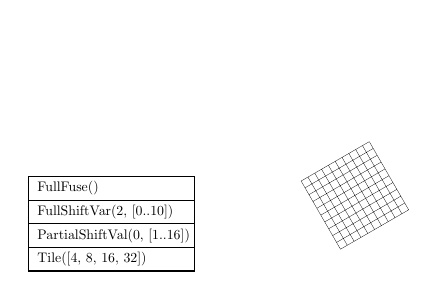
\begin{tikzpicture}

  %%% Begin Transformations %%%
  % XOXO
  \begin{scope}[xscale=2, yscale=1.5]
  \foreach [
    evaluate=\i as \xmaru using rand,
    evaluate=\i as \xbatsu using rand,
    evaluate=\i as \ymaru using rand,
    evaluate=\i as \ybatsu using rand,
    evaluate=\xmaru \ymaru as \smaru using (1.5-sqrt(\xmaru*\xmaru+\ymaru*\ymaru)),
    evaluate=\xbatsu \ybatsu as \sbatsu using (1.5-sqrt(\xbatsu*\xbatsu+\ybatsu*\ybatsu)),
    remember=\xmaru as \lxmaru (initially 0),
    remember=\ymaru as \lymaru (initially 0),
    ] \i in {1,2,...,40}{
    \node[scale=\sbatsu, opacity=1.2-\sbatsu] at (\xbatsu, \ybatsu) (batsu-\i) {\batsu};
    \node[scale=\smaru, opacity=1.2-\smaru] at (\xmaru, \ymaru) (maru-\i) {\maru};
  }
  \end{scope}
  \begin{scope}[rotate=30, xshift=0.3cm, yshift=-1.7cm]
  \draw[step=1mm, ultra thin] (0,0) grid (1,1);
  \end{scope}
  %%% End Transformations %%%
  %%% Begin Samples %%%
  \path node [
    scale=0.5,
    draw=black,
    fill=white,
    rectangle split,
    rectangle split parts=4,
    rectangle split part align=left,
  ] at (-1.8cm, -1cm)
    (legend) {         \textcolor{SpringGreen}{\CheckmarkBold}  FullFuse()
    \nodepart{two}     \textcolor{SpringGreen}{\CheckmarkBold}  FullShiftVar(2, [0..10])
    \nodepart{three}   \textcolor{SpringGreen}{\CheckmarkBold}  PartialShiftVal(0, [1..16])
    \nodepart{four}    \textcolor{SpringGreen}{\CheckmarkBold}  Tile([4, 8, 16, 32])
  }
  ;
  %%% End Samples %%%

\end{tikzpicture}
\end{document}
